%!TEX root = thesis.tex

\section{Experimental Assesment}

In order to be able to validate our theoretical results done in the previous parts, we used the help of a VSM setup to measure the magnetization of real macro-helices and calculate with it their demagnetization matrices. On parallel, the same macrohelices were modelled in COMSOL in order for the theoretical demagnetization matrix to be calculated.\\

\begin{figure}[ht]
	\centering
  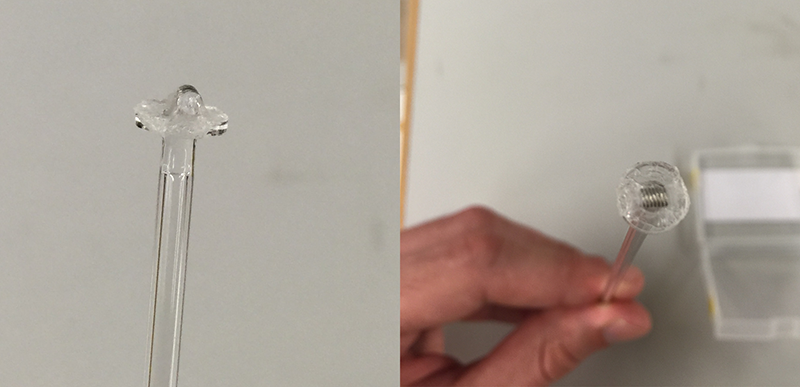
\includegraphics[width=0.8\textwidth]{Pictures/Macrohelix7.png}
	\caption{Handwired nickel macrohelix ($k=7$)}
	\label{fig:Macrohelix7}
\end{figure}

In Figure \ref{fig:Macrohelix7} we get an insight of the size of the helices we used. The helix was made of pure polycristalline nickel with a width of $d = 250$nm which was coiled around a non-magnetic M2.5 polymer screw and then attached to the measuring VSM probe using non-magnetic glue. The probe was then placed in the VSM setup (Figure \ref{fig:VSMSetup}). Through the shortening of the helix, we were able to do measurements for different number of coilings $k = 2, 3, 4$ and $7$.\\

\begin{figure}[ht]
	\centering
  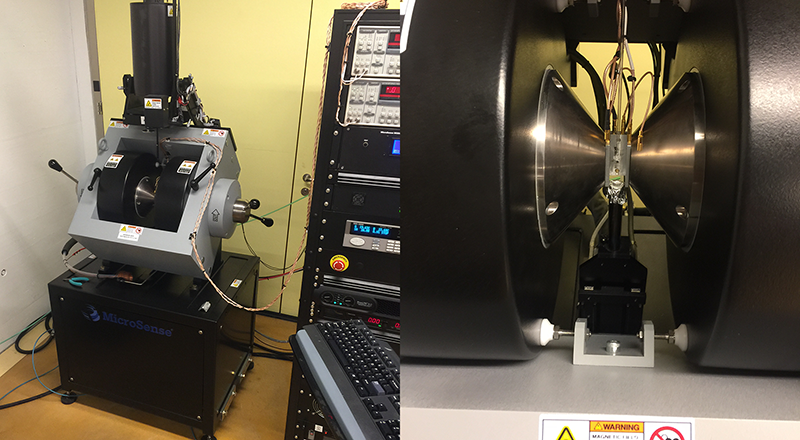
\includegraphics[width=0.8\textwidth]{Pictures/VSMSetup.png}
	\caption{VSM Setup for macrohelix measurements}
	\label{fig:VSMSetup}
\end{figure}

The VSM creates an approximately constant applied magnetic field in one direction to the probe and measures the magnetic moment in the direction of the applied field and the perpendicular direction on the plane parallel to the floor. 
We assumed  that both perpendicular radial directions of the helices are equal, such that we only have to measure one. With the VSM we measured one radial and the axial directions. We create a sweep that increases the applied field from zero to a point where the moment is practically saturated and then reduces it until it saturates in the opposite direction. Then it goes back to the saturate it in the original direction, thus completing the hysteresis loop.\\

\begin{figure}[ht]
	\centering
  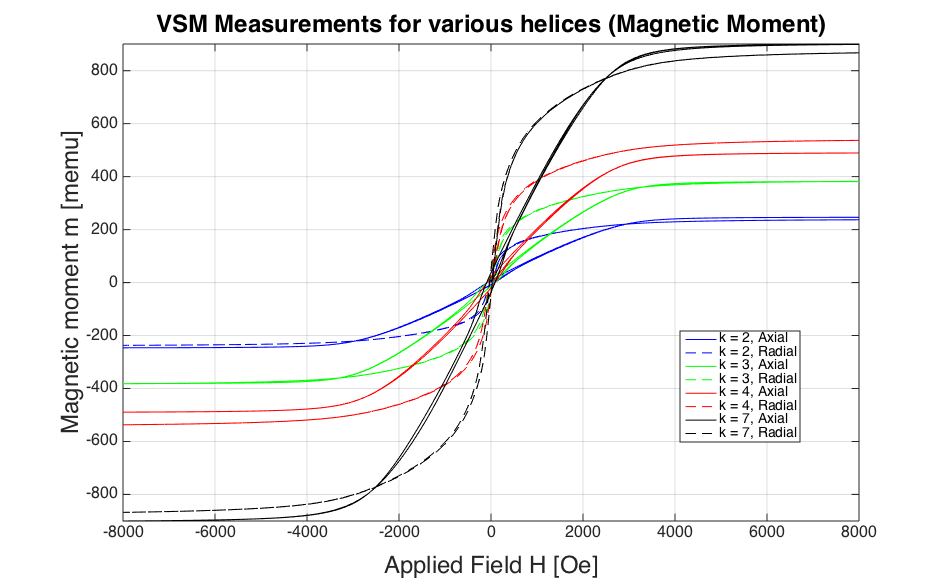
\includegraphics[width=1\textwidth]{Pictures/VSM_Moment.png}
	\caption{Magnetic moment vs. applied field for various coiling numbers $k$}
	\label{fig:VSM_Moment}
\end{figure}

For each the axial applied field and the radial applied field we extract two curves, one in axial and one in radial direction. We have thus four hysteresis loops per helix. An important step before continuing is to make sure that the curves all saturate at the appropiate moment. We calibrate, thus, using the, already given for nickel, mass specific saturation moment:

\begin{equation}
m_s = 54.97 \frac{\text{emu}}{g}
\end{equation}

We will take our integral equation for an applied field in both radial and in axial direction. Since we're dealing with low fields, we will take the linearization of $\chi_m(\textbf{H})$ for small $|\textbf{H}|$. 

%PROOF THAT MISSING VALUES DISSAPPEAR WHEN CALCULATING MISSALIGNMENT ANGLE

\begin{equation}
\frac{1}{\chi_m}\textbf{M}(\textbf{r}) = -N(\textbf{r})\textbf{M}(\textbf{r})  + \textbf{H}_\text{app}
\end{equation}

and we average it:

\begin{equation}
\frac{1}{\chi_m}\langle\textbf{M}(\textbf{r})\rangle = -\langle N(\textbf{r})\textbf{M}(\textbf{r})\rangle  + \textbf{H}_\text{app}
\end{equation}

this relation can be written in the following way\footnote{This is of course an assumption and it should be examined further in detailed to assess the correcness of it. See Appendix \ref{s:NMComparison} for a detailed comparison of both the exact case and the approximation}:

\begin{equation}
\frac{1}{\chi_m}\langle\textbf{M}(\textbf{r})\rangle \approx -\langle N(\textbf{r})\rangle\langle\textbf{M}(\textbf{r})\rangle  + \textbf{H}_\text{app}
\end{equation}
 We insert the relation between the total magnetic moment and the averaged magnetization:

\begin{equation}
\langle{M}(\textbf{r})\rangle = \frac{\textbf{m}}{V}
\end{equation}

We will write now $N$ for $\langle N(\textbf{r})\rangle$

\begin{equation}
\frac{1}{\chi_m}\frac{\textbf{m}}{V} = - N\frac{\textbf{m}}{V}  + \textbf{H}_\text{app}
\end{equation}

we construct our matrix with the axial and both radial applied fields and the correspondant measured magnetic dipoles:

\begin{equation}
\frac{1}{\chi_m}\frac{\textbf{1}}{V}m = - \frac{\textbf{1}}{V}N m  + H_\text{app}
\end{equation}

and we solve to $N$:

\begin{equation}
\frac{\textbf{1}}{V}\frac{1}{\chi_m}m = - \frac{\textbf{1}}{V}N m  + H_\text{app}
\end{equation}

\begin{equation}
N = V\; H_\text{app}\; m^{-1} - \frac{1}{\chi_m}I
\end{equation}

The important part here is that the measurements we do are only in the axial and one radial direction. Therefore we have to fill the missing parts of the matrices $m$ and $H_\text{app}$ with the assumption that both radial directions behave equally\\

In our case, we define $H_\text{app}$ defined in the following way:
\begin{equation}
H_\text{app} = [\textbf{H}_\text{ax}, \textbf{H}_\text{rad,1}, \textbf{H}_\text{rad,2}]
\end{equation}

Where:
\begin{equation}
H_\text{rad,2} =\frac{ \textbf{H}_\text{ax} \times \textbf{H}_\text{rad,1} }{|\textbf{H}_\text{ax} \times \textbf{H}_\text{rad,1}|}\;|\textbf{H}_\text{rad,1}|
\end{equation}

we then have the magnetization matrix obtained from the measurements:

\begin{equation}
m = [\textbf{m}_\text{ax},\textbf{m}_\text{rad,1},\textbf{m}_\text{rad,2}] = \left[\begin{array}{ccc}
m_\text{ax;ax} & m_\text{rad,1;ax} & m_\text{rad,2;ax} \\
m_\text{ax;rad,1} & m_\text{rad,1;rad,1} & m_\text{rad,2;rad,1}\\
m_\text{ax;rad,2} & m_\text{rad,1;rad,2} & m_\text{rad,2;rad,2}
\end{array}\right]
\end{equation}

where $m_\text{ax;ax}$,   $m_\text{rad,1;ax}$, $m_\text{ax;rad,1}$ and $m_\text{rad,1;rad,1}$ are known from the measurements. By assuming symmetry we assume the following for the rest of the values:

\begin{subequations}
\begin{equation}
m_\text{rad,2;ax} = m_\text{rad,1;ax} 
\end{equation}
\begin{equation}
m_\text{ax;rad,2} = m_\text{ax;rad,1} 
\end{equation}
\begin{equation}
 m_\text{rad,2;rad,2} = m_\text{rad,1;rad,1}
\end{equation}
\begin{equation}
m_\text{rad,1;rad,2} = m_\text{rad,2;rad,1} = 0
\end{equation}
\end{subequations}

The latter says that the magnetization in one radial direction when the applied field is in the other radial direction is zero. Altough locally it may not be zero, the symmetry of the helix as well as it having full coilings leads to a cancelling out in this direction \\

\subsection{The Apparent Susceptibility}

Although the whole theory to magnetism was already discussed in previous chapters, we find ourselves in the experimental area. As we saw before, a popular way of measuring magnetization is through a VSM, where the measurable variables are the applied field and the created magnetic torque.\\

Although the demagnetization matrix is the missing, body-dependant variable that completes the unique relation between an applied field and its magnetization, we will find a more direct and experimentally meaningful way of describing this relationship. For this, we start by showing our integral averaged equation for low fields, which simplifies to an algebraic equation (since the demagnetization factor is a constant matrix)\footnote{We will replace the '$\approx$' by '$=$' for simplification purposes as well as $N : = \langle N(\textbf{r})\rangle$ and $\textbf{M} : = \langle \textbf{M}(\textbf{r})\rangle$}:

\begin{equation}
\frac{1}{\chi_m}\textbf{M} =  -N\textbf{M}  + \textbf{H}_\text{app}
\end{equation}

we manipulate the equation ang get:
\begin{equation}
\left(\frac{1}{\chi_m}I+N\right) \textbf{M} = \textbf{H}_\text{app}
\end{equation}

and finally:
\begin{equation}
 \textbf{M} = \underbrace{\left(\frac{1}{\chi_m}I+N\right)^{-1}}_{:= \chi_a}\textbf{H}_\text{app}
\end{equation}

We see a constant, linear mapping between the applied field and the magnetization. We call this constant $\chi_a$, the apparent suceptibility, making an analogy to the structure of the magnetization within a body, which actually happens in each material point within the body with the magnetic suceptibility $\chi_m$:

\begin{equation}
 \textbf{M}(\textbf{r}) = \chi_m\textbf{H}(\textbf{r})
\end{equation}

Although this equation may make more sence from a physical point of view, it is impossible to use it directly to measure the magnetization of a body. We thus use, as mentioned before, the following\footnote{May the reader be aware of the fact that the magnetic susceptibility $\chi_m$, as it was mentioned before, is not only a function of the H-field and is in general a matrix. In this case we are dealing with the linearized version (constant) which can be written as a scalar instead of a diagonal matrix with identical diagonal values due to the crystal anisotropy}:

\begin{equation}
 \textbf{M} = \chi_a\textbf{H}_\text{app}
\end{equation}

\subsubsection{Comparison with the demagnetization matrix N}

From the above calculations we see the relation between the demagnetization matrix and the apparent susceptibility:

\begin{equation}\label{eq:chia}
\chi_a = \left(\frac{1}{\chi_m}I+N\right)^{-1}
\end{equation}

If we analyze the characteristics of both matrices we find two important characteristics:

The first one is that for highly magnetizable bodies, where the intrinsic magnetic susceptibility is high ($\chi_m >>1$) the following holds:

\begin{equation}
\chi_a \approx  N^{-1}
\end{equation}

The second, even more interesting one, is that both $\chi_a$ and $N$ (disregarding of the magnitude of $\chi_m$) share eigenvalues \footnote{See Appendix \ref{s:SameEigen} for proof} and therefore easy axes too. This means also, that we can analyze directly the easy axes of the demagnetization tensor $N_\text{av}$ to see how an applied field will magnetize the whole body. If the body has, in addition, a high magnetic susceptibility, i.e., $\chi_a \approx  N^{-1}$, then the eigenvalues are inverted.\\

If the demagnetization matrix and the apparent susceptibility share eigenvectors and have inverted eigenvalues (for the same eigenvector) means that the demagneti†zation factor has all the information about how the body will align and which directions will magnetize easier. This is the reason why, until now, we could always see out of the demagnetization matrix, which axes magnetize easier.\\

This gives us also a very important practical consequence: Since the magnetization $\textbf{M}$ is measurable one can easly determine the matrix $\chi_a$ since the applied field $\textbf{H}$ is also measurable. When $\chi_a$ is known one could theoretically calculate $\chi_m$ if the demagnetization factor is known (for example for a known shape), which is a much more intrinsic value (and not shape dependant). This scenario is only reachable when we're dealing with a shape that allows a uniform magnetization with low fields. That is the reason why ellipsoids are so important for measurements of this type.

\subsubsection{Calculation through VSM measurements}

Although at the beginning of this section, it was already shown how to calculate the demagnetization matrix out of the measurements. The apparent susceptibility is a construct that lets us work with a better sight of whats happening experimentally.\\

We showed before, that out of the VSM measurements we get four curves (Applied Field vs Magnetic Moment), two for every direction. We can then complement this two nine curves by doing the propper assumptions of symmetry in the helices.\\

Out of the definition of the apparent susceptibility acting as the map between the applied field and magnetization, It is not hard to see how we can calculate it directly from experments:

\begin{equation}
\chi_a = \frac{1}{V}mH_\text{app}^{-1}
\end{equation}

This brings us to the conclusion, that the single values in the $\chi_a$ matrix, are not more than the slopes of the single curves between applied field and magnetic moment from each direction measured in each direction.

\subsection{Measurement of intrinsic susceptibility $\chi_m$}


From now on, we want to be able to do a comparison between the VSM measurements and simulations.Equation \ref{eq:chia} states a relation between the demagnetization matrix and the apparent susceptibility matrix. The comparison is done by calculating the experimental demagnetization matrix for the body out of the measurements. This is done by reading the apparent susceptibility out of the VSM measurements, but the value of the intrinsic susceptibility $\chi_m$ has to be known beforehand in order to do this (otherwise there would be too many unknowns).\\

In order to measure the intrinsic susceptibility of Nickel, we used a polycristalline nickel sphere in the VSM (See Figure \ref{fig:NiSphere}).\\

\begin{figure}[ht]
	\centering
  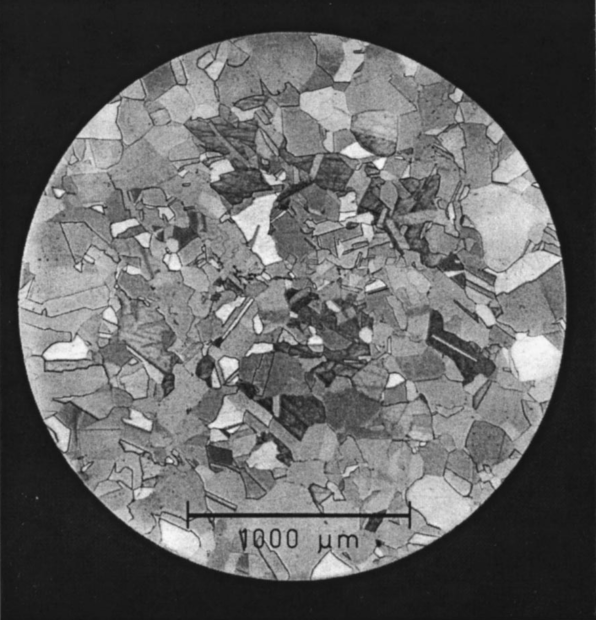
\includegraphics[width=0.4\textwidth]{Pictures/NiSphere.png}
	\caption{Cristalline structure of Nickel Sphere}
	\label{fig:NiSphere}
\end{figure}

We calculated afterwards its magnetic moment in the VSM. Figure \ref{fig:VSMNiSphere} shows the result.\\

\begin{figure}[ht]
	\centering
  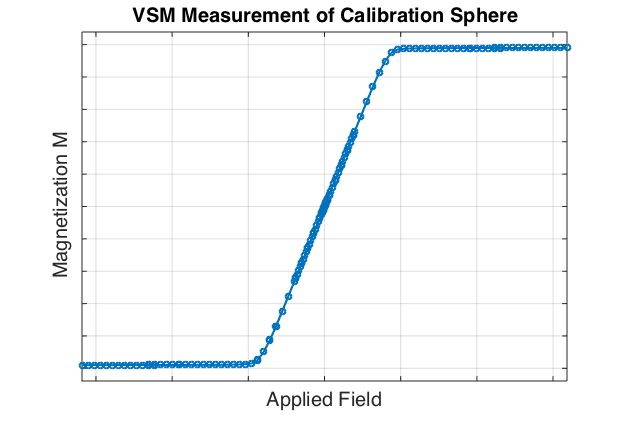
\includegraphics[width=0.8\textwidth]{Pictures/VSMNiSphere.png}
	\caption{Measurements of magnetic moment for a polycristalline nickel sphere}
	\label{fig:VSMNiSphere}
\end{figure}

A sphere always magnetizes uniformly for any kind of applied fields. Its demagnetization matrix therefore stays constant for low and high fields. Since, for high fields, the trace of the demagnetization matrix of any body sums up to   one, and a sphere is symmetric in all three directions the following holds:

\begin{equation}
N = \frac{1}{3}I
\end{equation}

For the same reason, the apparent susceptibility is the following:

\begin{equation}
\chi_a = \chi_{a,s}I
\end{equation}

Where $\chi_{a,s}$ is the slope of the curve until saturation (since it's a sphere, we would become that curve for every direction, therefore it stays constant). Writing down the definition of the apparent susceptibility and usign the demagnetization matrix for spheres, we get the following:

\begin{subequations}
\begin{equation}
\chi_a = \left(\frac{1}{\chi_m}I+N\right)^{-1}
\end{equation}
\begin{equation}
 \chi_{a,s}I = \left(\frac{1}{\chi_m}I+\frac{1}{3}I\right)^{-1}
\end{equation}
\end{subequations}

From which only one scalar equation remains relevant:

\begin{equation}
 \chi_{a,s} = \frac{1}{\frac{1}{\chi_m}+\frac{1}{3}}
\end{equation}

Which leads to the following:

\begin{equation}
 \chi_{m} = \frac{1}{\chi_{a,s}}-\frac{1}{3}
\end{equation}

In our measurements, the value was the following:

\begin{equation}
\chi_m \approx 24
\end{equation}


\subsection{Comparison with Simulations}

In the case of a perfect sphere, we saw from the graph, that the slope of the VSM measurement stays constant until its fully saturated. This is a special case which portrays the fact that the demagnetization matrix is constant for saturated as for non-saturated cases (since there is a unique algebraic transformation between $N$ and $\chi_a$. The interesting case, and crucial in this work, is to analyses and leave clear what happens for generic shapes (like helices) where the demagnetization matrix, and thus, the apparent susceptibility, is different for low fields as for high fields.\\

 To be more clear on this, lets analyze in FIgure \ref{fig:VSMExample} the graph of one example of the helices measured. Here we see, different than with the sphere, that the curve is not a constant slope that reaches saturation and then stays saturated, but rather goes smoothly from the unsaturated, linear case, to the saturated case. This case is very representative of the most general case and it leaves clear a very interesting point that is of core importance to the structure of this thesis: The apparent susceptibility, and therefore the demagnetization matrix, is dependent of the applied field and it is therefore of relevance to define the two limiting sections: low fields, when the slope is constant and high fields the exact point when the magnetization has reached a saturation point and it stays the same thereon.\\
 
 
 \begin{figure}[ht]
	\centering
  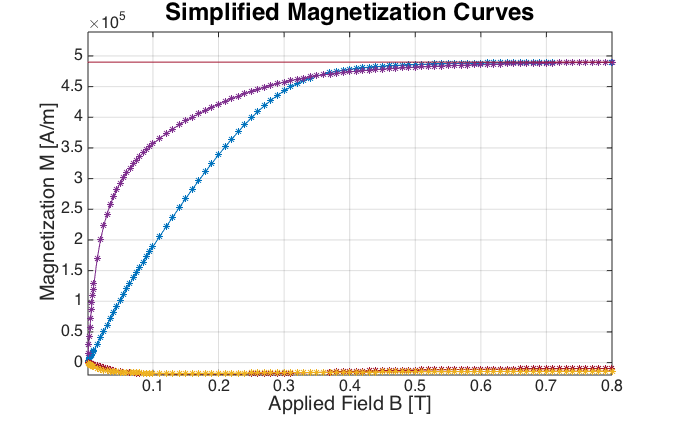
\includegraphics[width=0.8\textwidth]{Pictures/VSMExample.png}
	\caption{Calibrated VSM measurements of nickel macrohelix for positive applied fields. }
	\label{fig:VSMExample}
\end{figure}

 
 In the case of the sphere, the slopes are the same, but in the general case the challenge is to define both sections. The slope of the curve for low applied fields is not hard to find. As long as one takes small enough applied fields, a defined slope can be found for each curve. However, in the case of high fields, one has to define first the point where the saturation is reached and from that point on it stays saturated\footnote{May the reader be aware of this important convention: In this context, by slope, it is meant the slope of the line that goes from the origin to a certain point to the graph and not the slope in the sense of derivative}.\\
 
In order to be able to calculate the slopes of all curves to construct the apparent susceptibility and then the corresponding demagnetization matrix of each helix, we first have to do a meaningful definition of the point where the saturation happens, in order to calculate the slope at this point.\\
    
\begin{figure}[ht]
	\centering
  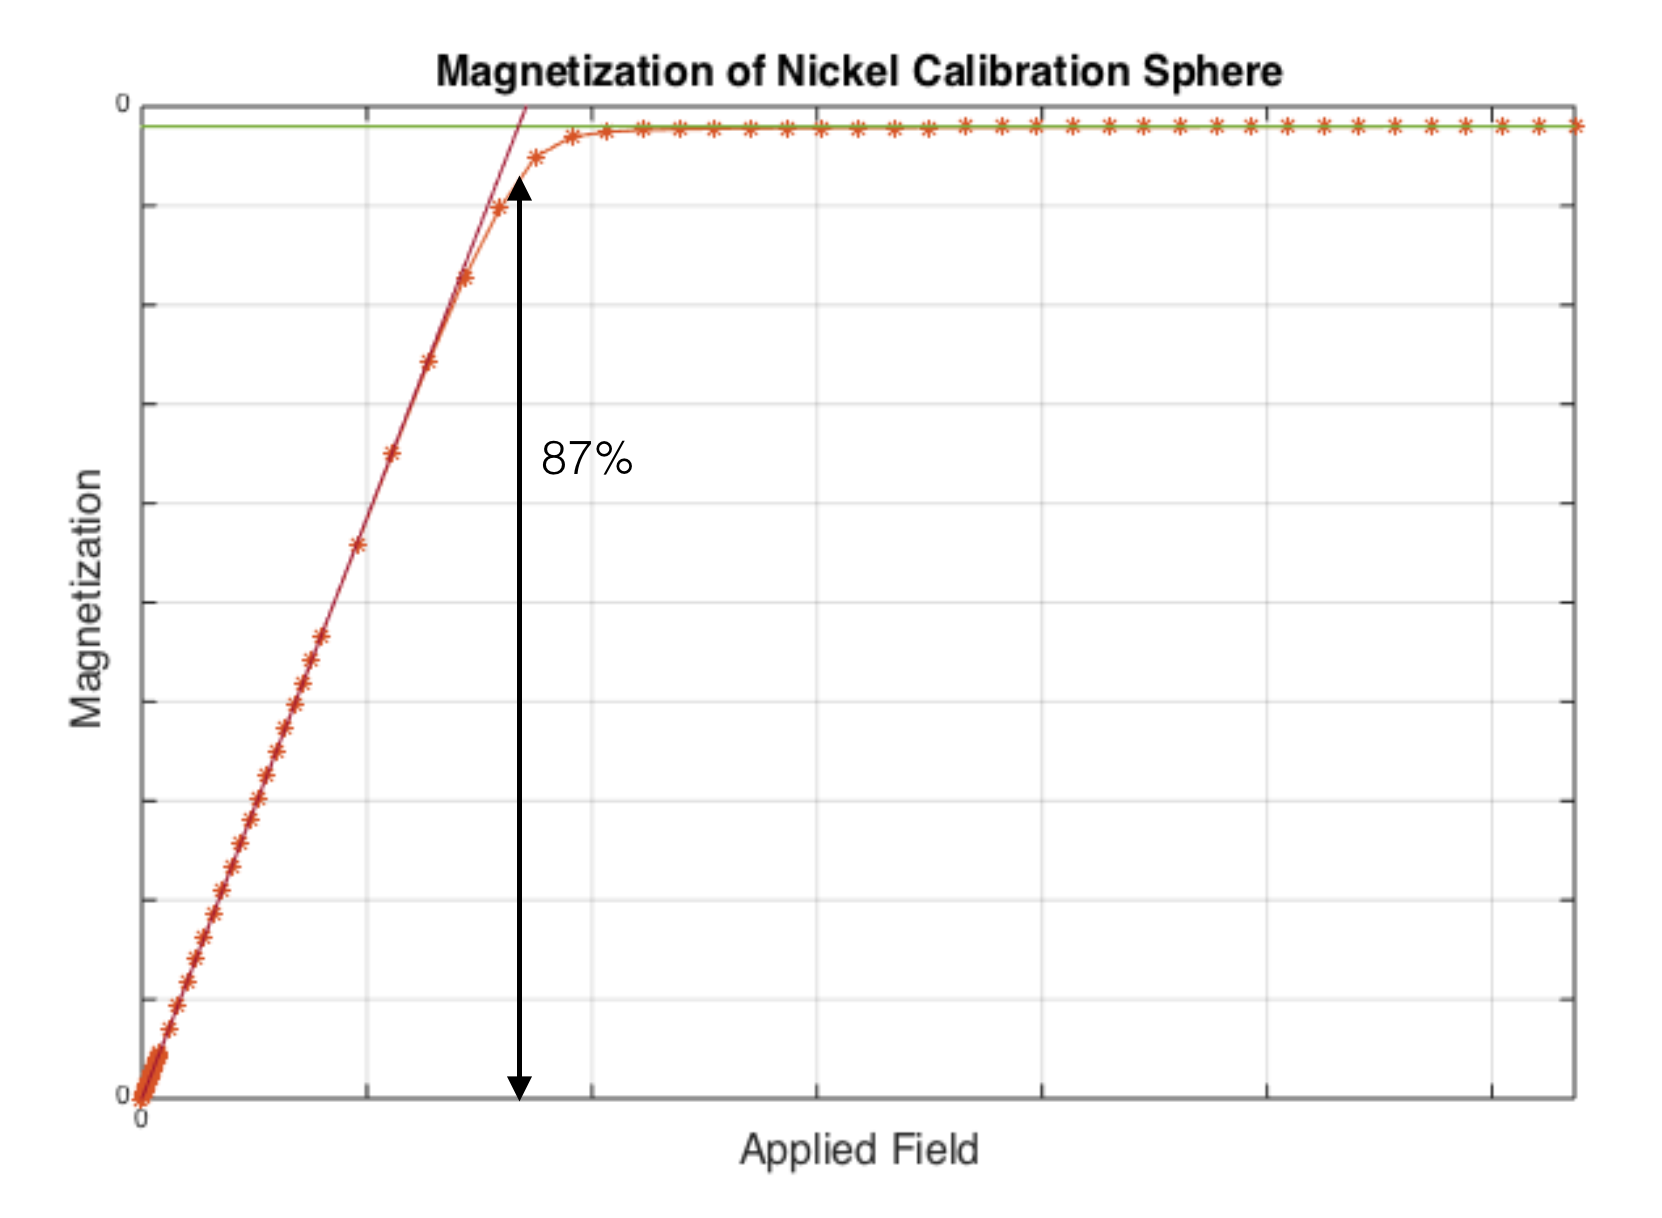
\includegraphics[width=0.8\textwidth]{Pictures/NiSphere_2.png}
	\caption{Measurements of magnetic moment for a polycrystalline nickel sphere with linearized trends}
	\label{fig:NiSphere_2}
\end{figure}

FIgure \ref{fig:NiSphere_2} shows the linearized trends of the low fields and the high field area of the nickel sphere. Ideally, since the nickel sphere is perfectly linear and magnetizes uniformly for any applied field, the demagnetization matrix and thus the apparent susceptibility (and thus the slope) should be constant until it saturates. Which means that the curve shouldn't be rounded, but rather stay perfectly linear until it saturates and then stay that way. In other words, the curve should never stop touching the trend lines.\\

The fact that this curve is not as it should in theory, can be used as criteria to do a quantitative comparison of how the real life case behaves compared to the theoretic one. In this case, we calculate the applied field in order for the theoretical curve to saturate, and then we calculate the percentage of saturation the actual curve actually achieves at this applied field. In this case, the ratio was $r = 87\%$.\\

This percentage will serve us as our criterium to analize and define saturation for the other helices. In other words, we will define the saturation point at the applied field, where the actual curve reaches $87\%$ of the saturation line for that specific helix. When doing that we will be able to calculate the slope of every curve and thus, the apparent susceptibility matrix of each helix and thus its demagnetization matrix, which we will then calculate with the simulations. \\


In Figure \ref{fig:NiHelix_Slopes} we see for $k = 2$ how the helix magnetization curves look like with the low field slopes as well as the saturation (high field) slopes defined there, where the curve achieves $r = 87\%$ of its saturation. For a complete assessment which includes all curves and calculations of demagnetization matrices and apparent susceptibilities please refer to Appendix \ref{s:ExperimentalResults}.\\

\begin{figure}[ht]
	\centering
  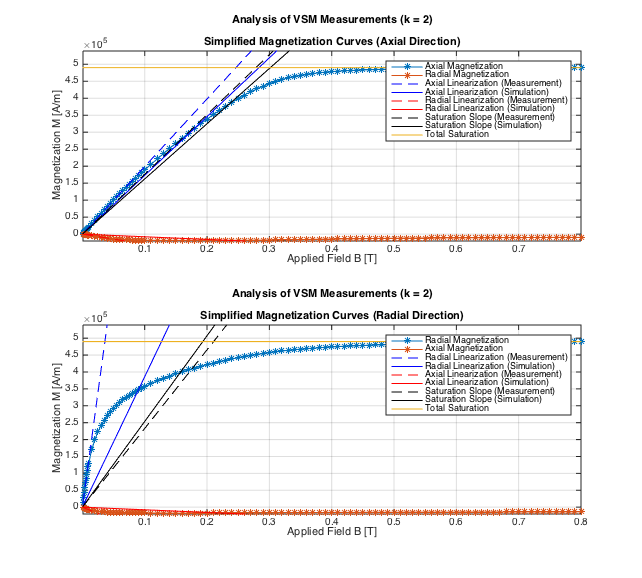
\includegraphics[width=1\textwidth]{Pictures/NiHelix_Slopes.png}
	\caption{Measurements of magnetic moment for a polycrystalline nickel helix with linearized trends (k = 2) and comparison with the simulated helices}
	\label{fig:NiHelix_Slopes}
\end{figure}

After analyzing the demagnetization matrices we see see that for $k=2, 3$ and $4$ we were able to capture the overall behavior of the magnetization for low and high fields. The easier axes to magnetize are the same in both results. For $k = 7$ the results are similar for low fields, but for high fields, we see a difference in the easier axes to magnetize between the simulation and the experiments. This is due to the fact that the diagonal values are very similar. \\

The results are satisfactory, considering the bold assumptions taken before. The factor contributing to the overall discrepancy between simulation and experiments could be not only human errors when coiling the macro helices, cutting them so the number of coiling turns is really a natural number and the alignment when putting the probe in the VSM, but also the assumption of same material composition between the sphere and the helices (which led to $r = 87\%$). \\

Also, one of the bold assumptions is the simplification of a hysteretic nonlinear curve to a single curve. Although the hysteresis is rather thing, the magnetization of the curve when magnetizing it from zero was not taken into consideration, but rather the complete loop curve, which was then averaged and centered such that it is a real symmetric curve that really crosses the origin. The major question would be, if this assumption is really meaningful, and it can only be answered depending of the application. Is the helix going to be re-magnetized or is it going to be magnetized from an absolutely neutral magnetization? These are questions that will have to be answered later depending on the specific application.

